\documentclass{beamer}
\usetheme{Warsaw}
\usepackage{polski}
\usepackage[utf8]{inputenc}
\usepackage[style=authortitle,backend=bibtex]{biblatex}
\addbibresource{bibliografia.bib}
\renewcommand{\footnotesize}{\tiny}

\title{Kształtowanie pola elektromagnetycznzego za pomocą elementów podfalowych}
\subtitle{Autoreferat}
\author{Marcin Stolarek}
\institute{Zakład Optyki Informacyjnej, Wydział Fizyki UW}
\date{\today}


\begin{document}


\frame{\titlepage}

\frame{\tableofcontents}

\section{Wielowarstwy metaliczno-dielektryczne}
\subsection{Pryzmat do obrazowania podfalowego}
\begin{frame}
	\begin{columns}
		\begin{column}{0.5\textwidth}
			\begin{figure}
				\includegraphics[width=\textwidth]{../images/multilayer/multilayer-3d.png}\\
		 	{\tiny Do projekotwania własności wielowarstwy wykorzystywaliśmy model efektywny, do badania własności symulacje metodami macierzowymi i FDTD.}

			\end{figure}
		\end{column}
		\begin{column}{0.5\textwidth}
			{\tiny Analiza własności wielowarstwy na podstawie wyników symulacji SMM i TMM prowadzona w języku optyki Fourierowskiej.}
			\begin{figure}
				\includegraphics[width=0.5\textwidth]{images/MTF-example.png}
				\includegraphics[width=0.6\textwidth]{images/MTF-perfect.png}
			\end{figure}
			\begin{figure}
				\includegraphics[width=0.5\textwidth]{images/Spoke.png}
				\includegraphics[width=0.5\textwidth]{images/Spoke-perfect.png}
			\end{figure}
		\end{column}
	\end{columns}
	\cite{PhysRevLett.85.3966}		
\end{frame}


\begin{frame}
	\begin{columns}
		\begin{column}{0.5\textwidth}
			Wykorzystanie pryzmatu miało umożliwić operację rzutowania również dla wiązek o rozmiarach podfalowych.
			\begin{figure}
				\includegraphics[width=\textwidth]{../images/multilayer/prism.png}
			\end{figure}
		\end{column}
		\begin{column}{0.5\textwidth}
			Wysoki współczynnik transmisji może być osiągnięty przez dopasowanie impedancyjne współczynników efektywnych do powietrza, w przypadku rezonansowego tunelowania wysoka transmisja moze byc uzyskana przez odpowiednie dobranie grubosci calej struktury do dlugosci fali.

		\end{column}
	\end{columns}
			\cite{scalora2001transparent}
		
\end{frame}

\begin{frame}[t]
	\begin{columns}
		\begin{column}{0.5\textwidth}
			\begin{figure}
				\includegraphics[width=\textwidth]{../images/multilayer/prism04.png} \\
				\includegraphics[width=\textwidth]{../images/multilayer/prism08.png} \\
			\end{figure}
		\end{column}
		\begin{column}{0.5\textwidth}
				\includegraphics[width=\textwidth]{../images/multilayer/prism12.png}\\
				Wydajność i FWHM wiązki wychodzącej zależą nie tylko od kąta łamiącego pryzmatu, ale i od przesunięcia wiązki wchodzącej, wskazując na brak możliwości stosowania modelu ośrodka efektywnego we wszystkich tego typu układach.
	
		\end{column}
	\end{columns}
		
\end{frame}

\subsection{Projektownie układów przez ray tracing}

\begin{frame}
	\begin{columns}
		\begin{column}{0.5\textwidth}
			\begin{figure}
				\includegraphics[angle=90,width=\textwidth]{../images/multilayer/konc_eps_mgr.png}\\
				\includegraphics[angle=90,width=\textwidth]{../images/multilayer/konc_ene_mgr.png}
			\end{figure}
		\end{column}
		\begin{column}{0.5\textwidth}
			\begin{itemize}
				\item Inżynierski model projektowania.
				\item Ograniczony silną dyfrakcją poza strukturą.
				\item Ścisłe modelowanie niezbędne.
			\end{itemize}
		
		\end{column}
	\end{columns}
		
\end{frame}

\begin{frame}
	\begin{columns}
		\begin{column}{0.5\textwidth}
			\begin{figure}
				\includegraphics[width=\textwidth]{../images/multilayer/konc_polk_poynt.png}\\
			\end{figure}
		\end{column}
		\begin{column}{0.5\textwidth}
				\includegraphics[width=\textwidth]{../images/multilayer/konc_coreshell_energy.png}\\
		\end{column}
	\end{columns}
		
\end{frame}

\begin{frame}
	\begin{columns}
		\begin{column}{0.5\textwidth}
			\begin{figure}
				\includegraphics[width=\textwidth]{../images/multilayer/plp-afm-chropo-1d.png}\\
				\includegraphics[width=\textwidth]{../images/multilayer/plp-afm-chropo.png}\\
			\end{figure}
		\end{column}
		\begin{column}{0.5\textwidth}
			Dla prowadzenia symulacji niezbędne było oddanie struktury wyspowej chropowatości powierzchni. \\ 
			Powierzchnie chropowate generowane były na podstawie danych z AFM, z zachowaniem widmowej gestosci mocy szumu.\\
		\end{column}
	\end{columns}
	\cite{Stolarek_2013}
		
\end{frame}

\begin{frame}
	\begin{columns}
		\begin{column}{0.5\textwidth}
				W symulacjach struktury w pelni gladkiej widoczna byla stojaca fala powierzchniowa na granicy metal-dielektryk, która zanika przy wprowadzeniu nawet minimalnej chropowatości -poprawa współczynnika transmisji.\\
				Chropowatość może poprawiać PSF.\\

		\end{column}
		\begin{column}{0.5\textwidth}
			\begin{figure}
				\includegraphics[width=\textwidth]{../images/multilayer/plp-chropo.png}\\
				\caption{ a,b - 430nm , c,d -490 nm}
			\end{figure}
		\end{column}
	\end{columns}
		
\end{frame}





\begin{frame}[t]
	\begin{columns}
		\begin{column}{0.5\textwidth}
			\begin{figure}
				\includegraphics[width=\textwidth]{../images/multilayer/oer-rms0.png}\\
				\includegraphics[width=\textwidth]{../images/multilayer/oer-rms01.png}\\
			\end{figure}
		\end{column}
		\begin{column}{0.5\textwidth}
				\includegraphics[width=\textwidth]{../images/multilayer/oer-rms05.png}\\
				Generalnie: nawet chropowatości na poziomie RMS ~ 1nm mogą znacząco zmniejszyć współczynnik transmisji przez wielowarstwę. \\
				 Szczególnie w przypadku dużej liczby warstw.
		\end{column}
	
	\end{columns}

	\cite{pastuszczak2013engineering}
		
\end{frame}

\subsection{Wpływ gładkości warstw}


\section{Siatki metalowe do kształtowania fali w THz}
\subsection{Antena dla detektora THz}
\begin{frame}
	\begin{columns}
		\begin{column}{0.5\textwidth}
			\centerline{$\frac{\lambda}{n_{eff}}=2\frac{W}{m}$}
			\begin{figure}
				\includegraphics[width=\textwidth]{../images/antenaThz/schemat.png}\\
				\includegraphics[width=\textwidth]{../images/antenaThz/rezonant_trans_f001.png}\\
			\end{figure}
		
		\end{column}
		\begin{column}{0.5\textwidth}
			\begin{figure}
				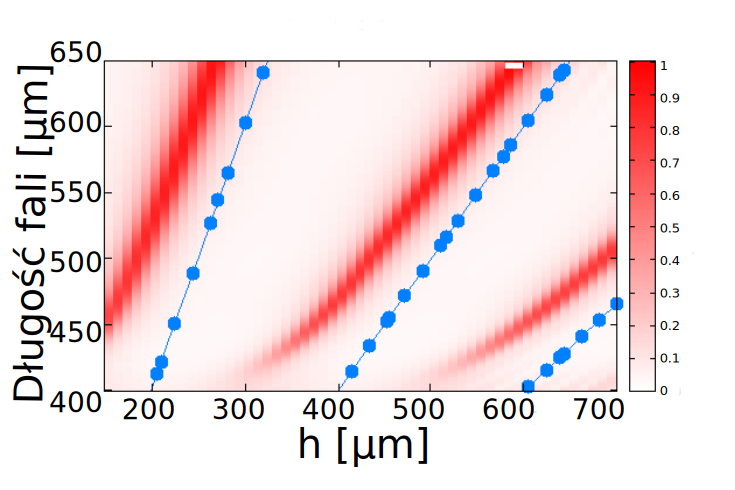
\includegraphics[width=\textwidth]{../images/antenaThz/rezonant_trans_f01.png}\\
				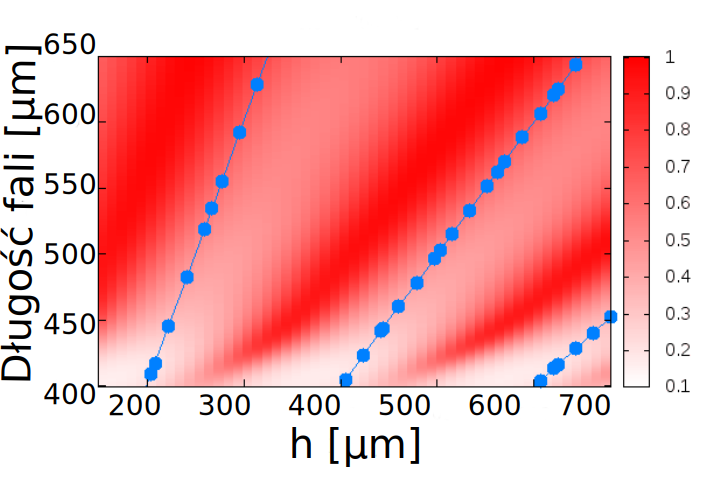
\includegraphics[width=\textwidth]{../images/antenaThz/rezonant_trans_f05.png}\\
			\end{figure}
		\end{column}
	\end{columns}
	\cite{martin2001theory}	
	
\end{frame}


\begin{frame}
	\begin{columns}
		\begin{column}{0.5\textwidth}
			\begin{figure}
				\includegraphics[width=\textwidth]{../images/antenaThz/con_src_l500.png}\\
				\includegraphics[width=\textwidth]{../images/antenaThz/con_src_l525.png}\\
				\includegraphics[width=\textwidth]{../images/antenaThz/con_src_l550.png}\\
			\end{figure}
		\end{column}
		\begin{column}{0.5\textwidth}
				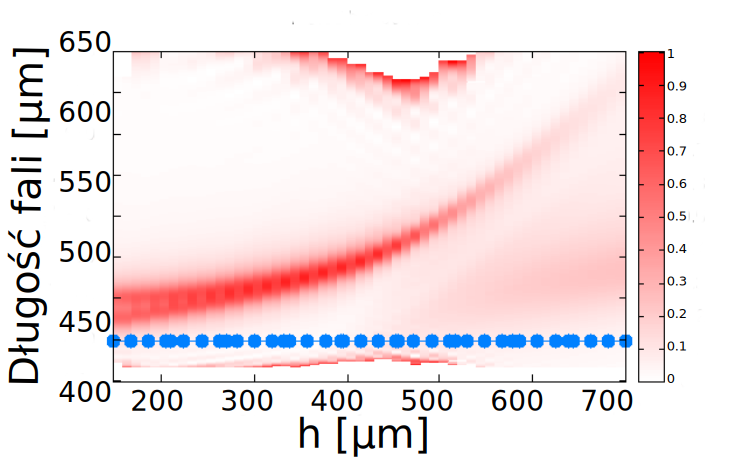
\includegraphics[width=\textwidth]{../images/antenaThz/rez_trans_L.png}\\
			Symulacje prowadzone byly z roznymi modelami materialowymi, zostalo potwierdzone, że w prowadzonych pracach metale mogą być przybliżane przy pomocy PEC.
		\end{column}
	\end{columns}
		
\end{frame}




\begin{frame}
	\begin{columns}

		\begin{column}{0.5\textwidth}
			\begin{figure}
				\includegraphics[width=\textwidth]{../images/antenaThz/gaas_mod_structure.png}\\
			\end{figure}
		\end{column}
		\begin{column}{0.5\textwidth}
			Ze względu na brak możliwości wykonania grubych siatek na podkładach GaAs zawierających detektory THz, zdecydowaliśmy się na wzbudzenie modu falowodowego w podkładzie. Symulacje pozytywnie zweryfikowały możliwości tak zaprojektowanej anteny.
		\end{column}
	\end{columns}
	\begin{figure}
		\includegraphics[width=\textwidth]{../images/antenaThz/final_stru.png}\\
	\end{figure}
		
\end{frame}



\subsection{Podwójne metalowe siatki dyfrakcyjne}
\begin{frame}
	\begin{columns}
		\begin{column}{0.5\textwidth}
			\begin{figure}
				\includegraphics[width=\textwidth]{../images/dmg/letters_eneden.png}
			\end{figure}
		\end{column}
		\begin{column}{0.5\textwidth}
			\begin{figure}
				\includegraphics[width=\textwidth]{../images/dmg/letters_schemat.png}
			\end{figure}
			Nie jest mozliwe uzyskanie transmisji asymetrycznej przez podwójne siatki metalowe w zerowym rzędzie ugięcia.
			
		\end{column}
	\end{columns}
	\cite{Stolarek:13}
		
\end{frame}

\begin{frame}
	\begin{columns}
		\begin{column}{0.5\textwidth}
			\begin{figure}
				\includegraphics[width=\textwidth]{../images/dmg/letters_exp_setup.png}\\
				\includegraphics[width=\textwidth]{../images/dmg/letters_spect.png}\\
			\end{figure}
		\end{column}
		\begin{column}{0.5\textwidth}
				\includegraphics[width=\textwidth]{../images/dmg/letters_exp.png}\\
		W porównaniu do poprzednich prac na temat DMG zakres długości fali charakteryzujący się transmisją asymetryczną został znacząco powiększony.
		\end{column}

	\end{columns}
		
\end{frame}

\begin{frame}
	\frametitle{Podniesienie kontrastu}
	\begin{columns}
		\begin{column}{0.5\textwidth}
			\begin{figure}
				\includegraphics[width=\textwidth]{../images/dmg/kontrast_schemat.png}\\
				\includegraphics[width=\textwidth]{../images/dmg/kontrast_maps.png}\\
			\end{figure}
		\end{column}
		\begin{column}{0.5\textwidth}
			\begin{figure}
				\includegraphics[width=\textwidth]{../images/dmg/kontrast_energy.png}\\
			\end{figure}
			Modifikacja rozmiarów otworów, oparta na zrozumieniu ich funkcji w procesie transmisji asymetrycznej pozwoliła na osiągnięcie wyższych współczynników transmisji i kontrastu dla propagacji w przeciwnych kierunkach.
		\end{column}
	\end{columns}
		
\end{frame}

\begin{frame}
	\frametitle{Polaryzacja radialna}
	\begin{columns}
		\begin{column}{0.5\textwidth}
			\begin{figure}
				\includegraphics[width=\textwidth]{../images/dmg/express_exp_setu.png}\\
			\end{figure}
		\end{column}
		\begin{column}{0.5\textwidth}
			\begin{figure}
				\includegraphics[width=\textwidth]{../images/dmg/express_siatki.png}\\
			\end{figure}
		\end{column}
	\end{columns}
	\cite{Yavorskiy:14}
		
\end{frame}

\begin{frame}
	Struktura zaprojektowana do:
	\begin{figure}
		\includegraphics[width=\textwidth]{../images/dmg/express_high_contrast.png}\\
	\end{figure}
	Eksperyment wykonany w "przeciwnym" kierunku:
	\begin{figure}
		\includegraphics[width=\textwidth]{../images/dmg/express_zarmata.png}\\
	\end{figure}
		
\end{frame}

\begin{frame}
	\begin{figure}
		\includegraphics[width=\textwidth]{../images/dmg/express_exp.png}\\
	\end{figure}
	Pomiary w eksperymencie wykazuję dobrą zgodność z modelowaniem. Oceniając wyniki eksperymentalne należy mieć na uwadze dużą wrażliwość układu na warunki zewnętrzne.
		
\end{frame}






\section{Realizacja PML przy pomocy wielowarstw}
\begin{frame}
	\begin{figure}
				\includegraphics[width=\textwidth]{../images/pml/oqe_schemat.png}
			\end{figure}

	\begin{columns}
		\begin{column}{0.5\textwidth}

		\end{column}
		\begin{column}{0.5\textwidth}

		\end{column}
	\end{columns}
	\cite{ania2015}	
\end{frame}

\begin{frame}
	\begin{figure}
				\includegraphics[width=\textwidth]{../images/pml/oqe_materials.png}
	\end{figure}
		
\end{frame}


\begin{frame} [t]
	\begin{columns}
		\begin{column}{0.5\textwidth}
			\begin{figure}
						\includegraphics[width=\textwidth]{../images/pml/oqe_materials.png}
			\end{figure}
			Realizacja materiałw z  $\mu \ne 1$ lub wzmocnieniem nie jest możliwa, konieczne jest przybliżenie propnowanego PML realnymi materiałami.			
		\end{column}
		\begin{column}{0.6\textwidth}
			\begin{figure}
						\includegraphics[width=0.9\textwidth]{../images/pml/oqe_reflection_kat.png}\\
			\end{figure}
				
		{\tiny	Dzięki oddzielnemu rozważaniu polaryzacji możemy wykluczyć zależność od części parametrów materiałowych. Nie możemy jednak wykluczyć zespolonego charakteru $\mu$.}

			\begin{figure}
						\includegraphics[width=0.9\textwidth]{../images/pml/oqe_reflection_kat_simp.png}
			\end{figure}

		\end{column}

	\end{columns}
		
\end{frame}


\begin{frame}
	\begin{columns}
			\begin{column}{0.5\textwidth}
			\begin{figure}
						\includegraphics[width=\textwidth]{../images/pml/oqe_trans_refl.png}
			\end{figure}
		\end{column}
		\begin{column}{0.5\textwidth}
			\begin{figure}
						\includegraphics[width=1.1\textwidth]{../images/pml/oqe_coreshell.png}
			\end{figure}
		\end{column}

	\end{columns}
		
\end{frame}

\section{}

\begin{frame}
	\frametitle{Dorobek naukowy}
	\begin{columns}
		\begin{column}{0.5\textwidth}
			h-index: 3 \\
			cytowań: 28 \\
			Seamless access to the PL-Grid e-infrastructure using UNICORE middleware (7 cytowań)\\
			Polish contribution to the worldwide LHC computing(4 cytowania)\\
		\end{column}
		\begin{column}{0.5\textwidth}
			\cite{Stolarek:13}\\
			\cite{Yavorskiy:14}\\
			\cite{ania2015}\\
			\cite{pastuszczak2013engineering}\\
		\end{column}
	\end{columns}
		
\end{frame}







\end{document}



%% Kawalki do przeklejania:
%% Ramka z kolumnami i obrazkiem:

